\section{Class Diagram cho task assignment module}
     \begin{figure}[H]
        \centering
        \rotatebox[]{90}{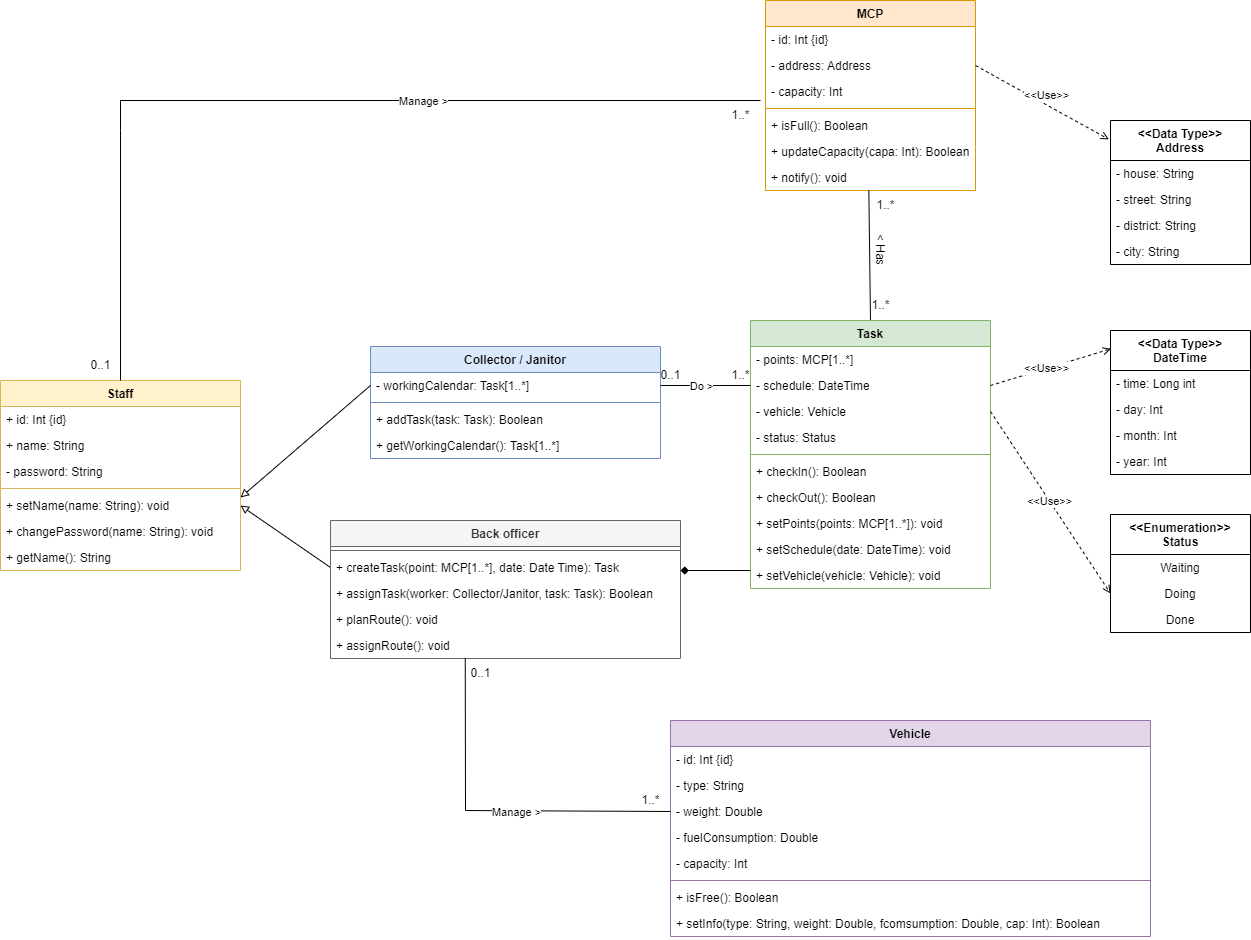
\includegraphics[height=11cm]{imgs/class diagram/class diagram.png}}
        \caption{Class diagram cho task assignment module}
    \end{figure}

    \newpage
    -Có tất cả 6 class trong module trên gồm có:
    \begin{enumerate}
        \item Class Staff:
        \begin{table}[htp]
            \begin{tabular}{|lll|}
                \hline
                \multicolumn{1}{|l|}{Class Name} & \multicolumn{2}{l|}{Staff}                                     \\ \hline
                \multicolumn{1}{|l|}{Inherit}    & \multicolumn{2}{l|}{None}                                      \\ \hline
                \multicolumn{3}{|c|}{\cellcolor[HTML]{FFFFC7}Attributes}                                          \\ \hline
                \multicolumn{1}{|l|}{int}        & \multicolumn{1}{l|}{id}               & Số định danh nhân viên \\ \hline
                \multicolumn{1}{|l|}{string}     & \multicolumn{1}{l|}{name}             & Tên nhân viên          \\ \hline
                \multicolumn{1}{|l|}{string}     & \multicolumn{1}{l|}{password}         & Mật khẩu đăng nhập     \\ \hline
                \multicolumn{3}{|c|}{\cellcolor[HTML]{FFFFC7}Methods}                                             \\ \hline
                \multicolumn{1}{|l|}{void}       & \multicolumn{1}{l|}{setName()}        & Đặt tên cho nhân viên  \\ \hline
                \multicolumn{1}{|l|}{void}       & \multicolumn{1}{l|}{changePassword()} & Đổi mật khẩu           \\ \hline
                \multicolumn{1}{|l|}{string}     & \multicolumn{1}{l|}{getName()}        & Lấy tên nhân viên      \\ \hline
                \multicolumn{3}{|c|}{\cellcolor[HTML]{FFFFC7}Relationships}                                       \\ \hline
                \multicolumn{1}{|l|}{Manage}     & \multicolumn{2}{l|}{Quản lý thông tin các MCP}                 \\ \hline
            \end{tabular}
        \end{table}
               
        \item Class Collector / Janitor:
        \begin{table}[htp]
            \begin{tabular}{|lll|}
                \hline
                \multicolumn{1}{|l|}{Class Name} & \multicolumn{2}{l|}{Collector/Janitor}                              \\ \hline
                \multicolumn{1}{|l|}{Inherit}    & \multicolumn{2}{l|}{Staff}                                          \\ \hline
                \multicolumn{3}{|c|}{\cellcolor[HTML]{FFFFC7}Attributes}                                               \\ \hline
                \multicolumn{1}{|l|}{Task{[}{]}} & \multicolumn{1}{l|}{workingCalendar}      & Lịch làm việc           \\ \hline
                \multicolumn{3}{|c|}{\cellcolor[HTML]{FFFFC7}Methods}                                                  \\ \hline
                \multicolumn{1}{|l|}{boolean}    & \multicolumn{1}{l|}{addTask()}            & Thêm task vào phần lịch \\ \hline
                \multicolumn{1}{|l|}{Task{[}{]}} & \multicolumn{1}{l|}{getWorkingCalendar()} & Lấy, xem lịch làm việc  \\ \hline
                \multicolumn{3}{|c|}{\cellcolor[HTML]{FFFFC7}Relationships}                                            \\ \hline
                \multicolumn{1}{|l|}{Do}         & \multicolumn{2}{l|}{Collector và Janitor thực hiện task}            \\ \hline
            \end{tabular}
        \end{table}
           
        \item Class Back officer:
        \begin{table}[htp]
            \begin{tabular}{|lll|}
                \hline
                \multicolumn{1}{|l|}{Class Name}  & \multicolumn{2}{l|}{Back officer}                                     \\ \hline
                \multicolumn{1}{|l|}{Inherit}     & \multicolumn{2}{l|}{Staff}                                            \\ \hline
                \multicolumn{3}{|c|}{\cellcolor[HTML]{FFFFC7}Attributes}                                                  \\ \hline
                \multicolumn{3}{|c|}{\cellcolor[HTML]{FFFFC7}Methods}                                                     \\ \hline
                \multicolumn{1}{|l|}{Task}        & \multicolumn{1}{l|}{createTask()} & Tạo task                          \\ \hline
                \multicolumn{1}{|l|}{boolean}     & \multicolumn{1}{l|}{assignTask()} & Gán task cho collector và janitor \\ \hline
                \multicolumn{1}{|l|}{void}        & \multicolumn{1}{l|}{planRoute()}  & Tạo tuyến đường                   \\ \hline
                \multicolumn{3}{|c|}{\cellcolor[HTML]{FFFFC7}Relationships}                                               \\ \hline
                \multicolumn{1}{|l|}{Manage}      & \multicolumn{2}{l|}{Quản lý thông tin phương tiện}                    \\ \hline
                \multicolumn{1}{|l|}{Composition} & \multicolumn{2}{l|}{Bao gồm task}                                     \\ \hline
            \end{tabular}
        \end{table}
   
        \newpage
           
        \item Class Task:
        \begin{table}[htp]
            \begin{tabular}{|lll|}
                \hline
                \multicolumn{1}{|l|}{Class Name} & \multicolumn{2}{l|}{Task}                                          \\ \hline
                \multicolumn{1}{|l|}{Inherit}    & \multicolumn{2}{l|}{None}                                          \\ \hline
                \multicolumn{3}{|c|}{\cellcolor[HTML]{FFFFC7}Attributes}                                              \\ \hline
                \multicolumn{1}{|l|}{MCP{[}{]}}  & \multicolumn{1}{l|}{points}        & Danh sách các MCP của task    \\ \hline
                \multicolumn{1}{|l|}{DateTime}   & \multicolumn{1}{l|}{schedule}      & Thời gian làm cho task        \\ \hline
                \multicolumn{1}{|l|}{Vehicle}    & \multicolumn{1}{l|}{vehicle}       & Phương tiện dùng cho task     \\ \hline
                \multicolumn{1}{|l|}{Status}     & \multicolumn{1}{l|}{status}        & Trạng thái của task           \\ \hline
                \multicolumn{3}{|c|}{\cellcolor[HTML]{FFFFC7}Methods}                                                 \\ \hline
                \multicolumn{1}{|l|}{boolean}    & \multicolumn{1}{l|}{checkIn()}     & check in task                 \\ \hline
                \multicolumn{1}{|l|}{boolean}    & \multicolumn{1}{l|}{checkOut()}    & check out task                \\ \hline
                \multicolumn{1}{|l|}{void}       & \multicolumn{1}{l|}{setPoints()}   & Đặt danh sách MCP cho task    \\ \hline
                \multicolumn{1}{|l|}{void}       & \multicolumn{1}{l|}{setSchedule()} & Đặt lịch cho task             \\ \hline
                \multicolumn{1}{|l|}{void}       & \multicolumn{1}{l|}{setVehicle()}  & Đặt phương tiện dùng cho task \\ \hline
                \multicolumn{3}{|c|}{\cellcolor[HTML]{FFFFC7}Relationships}                                           \\ \hline
                \multicolumn{1}{|l|}{Has}        & \multicolumn{2}{l|}{Mang thông tin các MCP}                        \\ \hline
            \end{tabular}
        \end{table}
           
           
        \item Class Vehicle:
        \begin{table}[htp]
            \begin{tabular}{|lll|}
                \hline
                \multicolumn{1}{|l|}{Class Name} & \multicolumn{2}{l|}{Vehicle}                                                               \\ \hline
                \multicolumn{1}{|l|}{Inherit}    & \multicolumn{2}{l|}{None}                                                                  \\ \hline
                \multicolumn{3}{|c|}{\cellcolor[HTML]{FFFFC7}Attributes}                                                                      \\ \hline
                \multicolumn{1}{|l|}{int}        & \multicolumn{1}{l|}{id}              & Số định danh phương tiện                            \\ \hline
                \multicolumn{1}{|l|}{string}     & \multicolumn{1}{l|}{type}            & Loại phương tiện                                    \\ \hline
                \multicolumn{1}{|l|}{double}     & \multicolumn{1}{l|}{weight}          & Khối lượng phương tiện                              \\ \hline
                \multicolumn{1}{|l|}{double}     & \multicolumn{1}{l|}{fuelConsumption} & Mức tiêu thụ nhiên liệu                             \\ \hline
                \multicolumn{1}{|l|}{int}        & \multicolumn{1}{l|}{capacity}        & Sức chứa của phương tiện                            \\ \hline
                \multicolumn{3}{|c|}{\cellcolor[HTML]{FFFFC7}Methods}                                                                         \\ \hline
                \multicolumn{1}{|l|}{boolean}    & \multicolumn{1}{l|}{isFree()}        & Kiểm tra phương tiện có đang được sử dụng hay không \\ \hline
                \multicolumn{1}{|l|}{boolean}    & \multicolumn{1}{l|}{setInfo()}       & Đặt thông tin cho phương tiện                       \\ \hline
                \multicolumn{3}{|c|}{\cellcolor[HTML]{FFFFC7}Relationships}                                                                   \\ \hline
            \end{tabular}
        \end{table}
           
        \newpage
        \item Class MCP:
        \begin{table}[htp]
            \begin{tabular}{|lll|}
                \hline
                \multicolumn{1}{|l|}{Class Name} & \multicolumn{2}{l|}{MCP}                                                            \\ \hline
                \multicolumn{1}{|l|}{Inherit}    & \multicolumn{2}{l|}{None}                                                           \\ \hline
                \multicolumn{3}{|c|}{\cellcolor[HTML]{FFFFC7}Attributes}                                                               \\ \hline
                \multicolumn{1}{|l|}{int}        & \multicolumn{1}{l|}{id}               & Số định danh cho MCP                        \\ \hline
                \multicolumn{1}{|l|}{Address}    & \multicolumn{1}{l|}{address}          & Địa chỉ của MCP                             \\ \hline
                \multicolumn{1}{|l|}{int}        & \multicolumn{1}{l|}{capacity}         & Sức chứa của MCP                            \\ \hline
                \multicolumn{1}{|l|}{int}        & \multicolumn{1}{l|}{capacity}         & Sức chứa của phương tiện                    \\ \hline
                \multicolumn{3}{|c|}{\cellcolor[HTML]{FFFFC7}Methods}                                                                  \\ \hline
                \multicolumn{1}{|l|}{boolean}    & \multicolumn{1}{l|}{isFull()}         & Kiểm tra MCP có đang đầy chỗ chứa hay không \\ \hline
                \multicolumn{1}{|l|}{boolean}    & \multicolumn{1}{l|}{updateCapacity()} & Cập nhật lại sức chứa MCP                   \\ \hline
                \multicolumn{1}{|l|}{void}       & \multicolumn{1}{l|}{notify()}         & Thông báo khi MCP hết sức chứa              \\ \hline
                \multicolumn{3}{|c|}{\cellcolor[HTML]{FFFFC7}Relationships}                                                            \\ \hline
            \end{tabular}
        \end{table}
\end{enumerate}